We implemented a chat using NodeJs and the node-serialport library.
The chat has a command line interface and offers the following functionalities:
\begin{itemize}

  \item configure used device
  \item configure retrans, difs, cwmin and cwmax with command line parameters
  \item logging to a .csv file
  \item fallback to default values if nothing provided
  \item broadcast and private messages
  \item "spam" mode to generate saturation traffic
\end{itemize}
Screenshots:
\begin{figure}[htp]
\centering
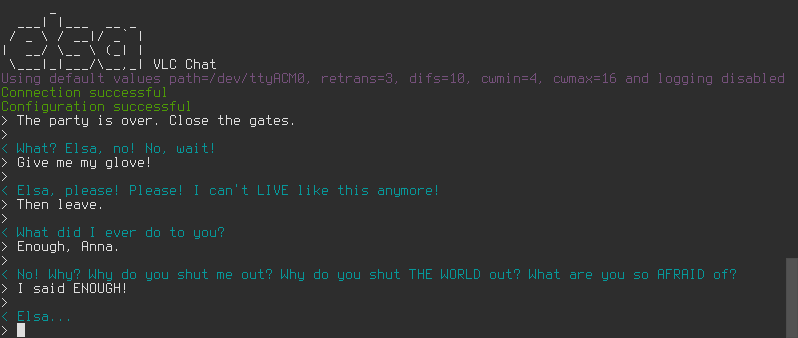
\includegraphics[width=\textwidth]{../img/elsa_1.png}
\caption{}
\label{}
\end{figure}
\begin{figure}[htp]
\centering
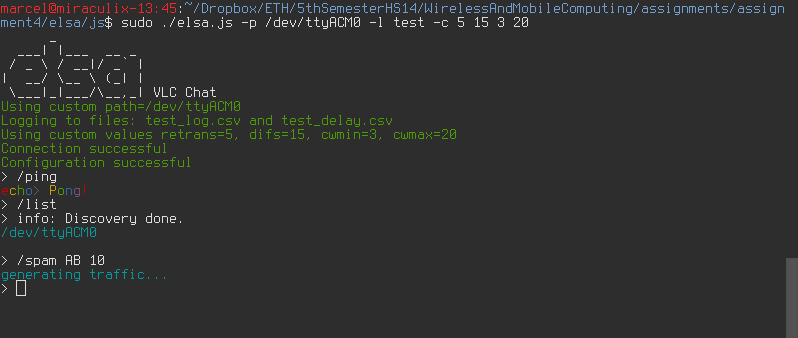
\includegraphics[width=\textwidth]{../img/elsa_2.png}
\caption{}
\label{}
\end{figure}
\begin{figure}[htp]
\centering
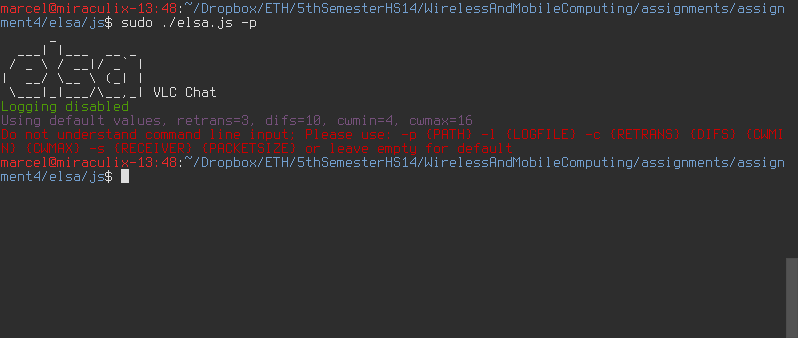
\includegraphics[width=\textwidth]{../img/elsa_3.png}
\caption{}
\label{}
\end{figure}

Code see attached zip file code.zip.